\documentclass[border=8pt]{standalone}
% Shared preamble for IronClaw thesis figures (standalone TikZ).
\renewcommand{\familydefault}{\sfdefault}
\usepackage{tikz}
\usetikzlibrary{arrows.meta,positioning,calc,fit,backgrounds,shapes.geometric,shapes.misc}

% IronClaw palette (matches slides.tex)
\definecolor{IronDark}{HTML}{1A2B3C}
\definecolor{IronBlue}{HTML}{2E86AB}
\definecolor{IronTeal}{HTML}{06A77D}
\definecolor{IronOrange}{HTML}{F18F01}
\definecolor{IronRed}{HTML}{C73E1D}
\definecolor{IronLight}{HTML}{F4F7F9}
\definecolor{IronGray}{HTML}{5D6D7E}

\tikzset{
  figtitle/.style={font=\large\bfseries\color{IronDark}, align=center},
  hostbox/.style={draw=IronBlue, rounded corners=5pt, fill=IronBlue!8,
                  line width=1pt, align=center, font=\small\color{white}},
  hostfill/.style={draw=IronBlue, rounded corners=4pt, fill=IronBlue,
                   line width=0.8pt, align=center, font=\small\color{white},
                   text width=3.1cm, minimum height=0.85cm},
  guestfill/.style={draw=IronOrange, rounded corners=4pt, fill=IronOrange!85,
                    line width=0.8pt, align=center, font=\small\color{white},
                    text width=3.1cm, minimum height=0.85cm},
  guestsoft/.style={draw=IronOrange, rounded corners=4pt, fill=IronOrange!25,
                    line width=0.8pt, align=center, font=\small\color{IronDark},
                    text width=3.1cm, minimum height=0.75cm},
  arrow/.style={-{Latex[length=2.6mm,width=2mm]}, line width=0.9pt, IronDark},
  biarrow/.style={{Latex[length=2.6mm,width=2mm]}-{Latex[length=2.6mm,width=2mm]},
                  line width=0.9pt, IronDark},
  note/.style={font=\footnotesize\color{IronGray}, align=center},
}

\begin{document}
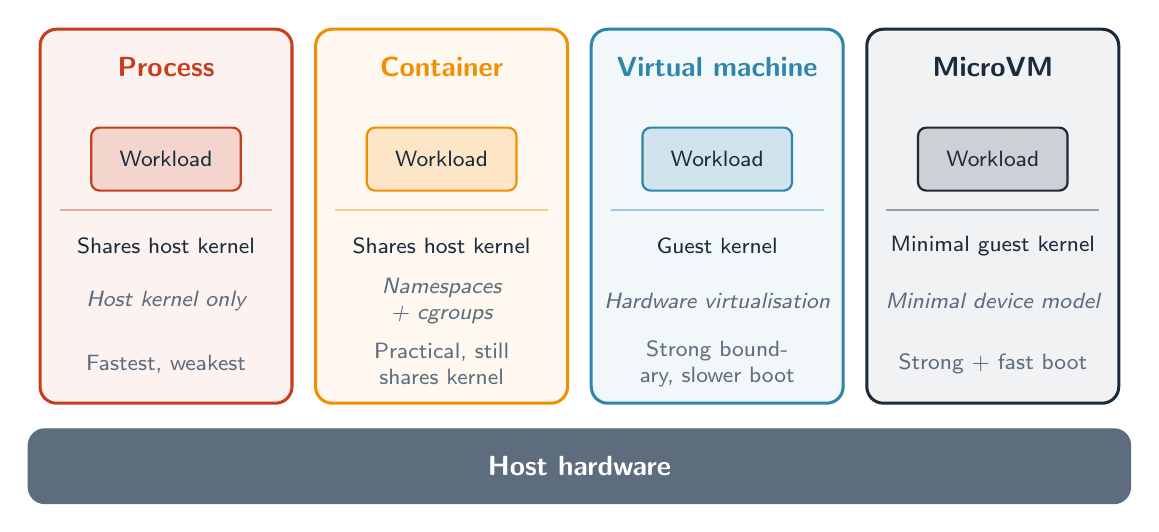
\begin{tikzpicture}

  % \pillar{x}{color}{title}{kernel line}{mechanism (italic)}{verdict (gray)}
  \newcommand{\pillar}[6]{%
    \begin{scope}[on background layer]
      \draw[draw=#2, line width=1.1pt, rounded corners=6pt, fill=#2!6]
        (#1-1.6,-1.25) rectangle (#1+1.6,3.5);
    \end{scope}
    \node[font=\normalsize\bfseries\color{#2}] at (#1,3.02) {#3};
    \node[draw=#2, fill=#2!22, rounded corners=3pt, line width=0.8pt,
          minimum width=1.9cm, minimum height=0.8cm,
          font=\footnotesize\color{IronDark}] at (#1,1.85) {Workload};
    \draw[#2!45, line width=0.6pt] (#1-1.35,1.2) -- (#1+1.35,1.2);
    \node[font=\footnotesize\color{IronDark}, align=center, text width=2.9cm] at (#1,0.75) {#4};
    \node[font=\footnotesize\itshape\color{IronGray}, align=center, text width=2.9cm] at (#1,0.05) {#5};
    \node[font=\footnotesize\color{IronGray}, align=center, text width=2.9cm] at (#1,-0.75) {#6};
  }

  \pillar{-5.25}{IronRed}{Process}{Shares host kernel}{Host kernel only}{Fastest, weakest}
  \pillar{-1.75}{IronOrange}{Container}{Shares host kernel}{Namespaces + cgroups}{Practical, still shares kernel}
  \pillar{ 1.75}{IronBlue}{Virtual machine}{Guest kernel}{Hardware virtualisation}{Strong boundary, slower boot}
  \pillar{ 5.25}{IronDark}{MicroVM}{Minimal guest kernel}{Minimal device model}{Strong + fast boot}

  % shared host hardware
  \node[draw=IronGray, fill=IronGray, text=white, rounded corners=6pt,
        minimum width=14.0cm, minimum height=0.95cm, font=\normalsize\bfseries]
        at (0,-2.05) {Host hardware};

\end{tikzpicture}
\end{document}
